%=============================================================================
%
%     Artikel
%
%=============================================================================

%-------------------------------  PREAMBLE  ----------------------------------

\documentclass[a4paper,12pt,german]{article}

\usepackage[german]{babel}
\usepackage[latin1]{inputenc} 
\usepackage{graphicx}
\usepackage{color}
\usepackage{listings}
%\usepackage{nn,rl,useful}

\oddsidemargin0.5cm
\textwidth15.5cm
\topmargin0cm
\textheight23cm
%\headsep2cm
\setlength{\parskip}{1ex plus0.5ex minus0.5ex} % Abstand zwischen zwei Absaetzen
\parindent0cm % Einrueckung der ersten Zeile eines Absatzes

\newcommand{\cls}{{CLS$^2$ }}
\newcommand{\clsquare}{{CLS$^2$ }}
\newcommand{\main}{{main.c }}
\newcommand{\clsdir}{{\$CLS\_DIR}}
\newcommand{\Xplus}{{${\cal X}^+$}}
\newcommand{\Xminus}{{${\cal X}^-$}}
\newcommand{\Xwork}{{${\cal X}^{work}$}}
\newcommand{\Xinit}{{${\cal X}^{init}$}}
\newcommand{\ite}{\begin{itemize}}
\newcommand{\eti}{\end{itemize}}

\newcommand{\Todo}[1]{{\bf Todo:} #1}

\definecolor{myColor}{rgb}{0.9,0.9,0.9}
\definecolor{MyGray}{rgb}{0.92,0.93,0.94}
\definecolor{MyGray2}{rgb}{0.82,0.93,0.94}
\definecolor{MyGray3}{rgb}{0.92,0.83,0.94}

\makeatletter\newenvironment{graybox}{%
   \begin{lrbox}{\@tempboxa}\begin{minipage}{0.9\columnwidth}}{\end{minipage}\end{lrbox}%
   \colorbox{MyGray}{\usebox{\@tempboxa}}
}\makeatother

\newcommand{\anmerkung}[2]{\vspace*{0.01cm}\begin{center}\begin{graybox}{\bf #1 :\\}{\em #2}\end{graybox}\end{center}\vspace*{0.1cm}}



%---------------------------------  DOCUMENT  --------------------------------
\begin{document}

\title{\vspace*{-5cm}\cls (clsquare) 4.0 - A Closed Loop Simulation System\\
{\normalsize freely available at: http://clss.sf.sourceforge.net}}
\author{Martin Riedmiller, Roland Hafner, Sascha Lange, Manuel Blum\\Machine Learning Lab\\
Albert-Ludwigs-University Freiburg}

%\date{\vspace*{2cm}\centerline{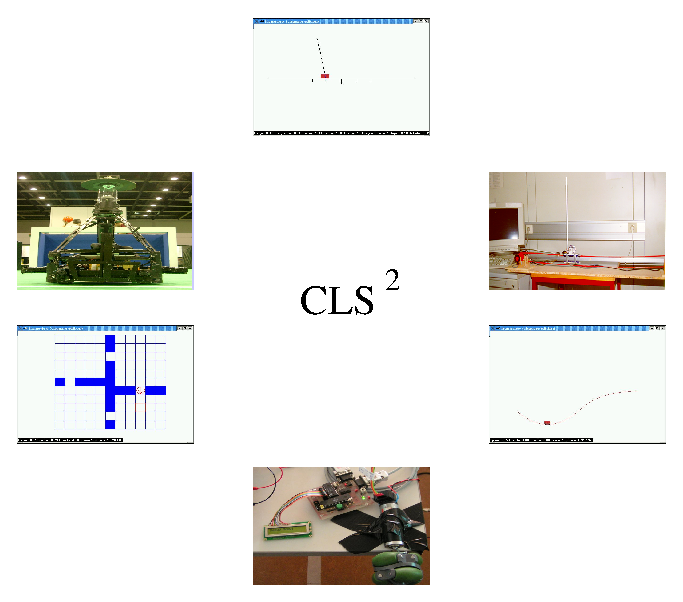
\includegraphics[width=10cm]{clslogo.eps}}}


\maketitle

\centerline{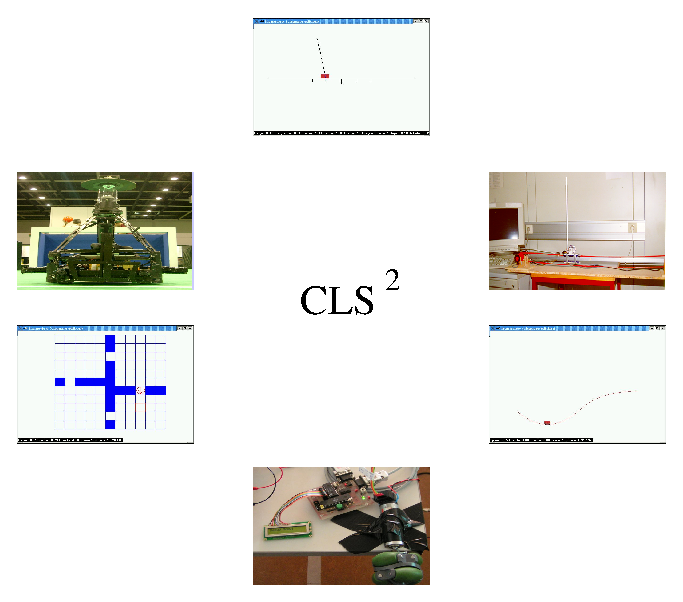
\includegraphics[width=7cm]{clslogo}}


\newpage

\section{Introduction to \cls}

\subsection{The idea}

\cls (pronounced: clsquare)  provides a standardized framework for running
controllers and plants in a closed control loop. It is meant as a
training and testing framework for both classical and learning controllers.
In particular, by providing all necessary features to define Markovian Decision
Processes (MDPs), it is particularly suited for reinforcement learning (RL)
controllers. By straight-forward configuration via a config file mechanism, 
\cls allows the easy combination of controllers and plants.

\cls comes with a considerable number of standard plants (or
'environments') taken both from the RL literature and from the
classical control literature. Additional modules provide interfaces to
graphical viewers or allow to do statistics, in order to document
learning behavior.
 
Special care is taken on the easy integration of new plants and
controllers. By this, we want to encourage people to contribute to the
system by sharing their plants and controllers.

Features:

\ite
\item provides a standardized control loop with built-in documentation facilities as used in typical 
reinforcement learning and classical control tasks
\item easy combination of different plants and controllers via definition in a configuration file
\item equal treatment of real and simulated plants
\item standardized, external graphical interface
\item lean interfaces for plants and controllers using standard data types only, allow a quick
migration to and from \cls from and to other software environments
\item prototypical implementations of plant and controller make the implementation of new
systems easy
\item careful definition of the information available to the distinct modules 
make the framework compatible to classical control theory while also allowing
to address problems tackled in reinforcement learning research (like e.g.
the realization of partial observable MDPs, POMDPs).
\eti

\subsection{A first glance at the concepts}

\ite
\item implements a discrete time closed loop control framework
\item two main modules: controller and plant. The controller takes as
  input information about the current state (might be incomplete and/
  or noisy) and outputs an action. The plant takes as input its
  current state and the current action, performs a transition and
  provides information about the next state.
\item optional modules to realize advanced concepts: reward, observer.
reward computes the reward for a certain state transition and determines, whether
a terminal state is reached. The reward module therefore provides the information
needed to define an MDP. The reward module might delegate its computation to the
plant module (e.g. if information is needed, that is only available within the
plant directly). The observer module realizes the concept of an observer known
from classical control theory. In its simplest form, it directly maps the sensor
information from the plant to an 'observed state'. However, it might also be used
to realize more sophisticated concepts, like e.g. gathering historical information.
\item service modules: input, output, statistics, graphics
\item all modules are called once per time step to fulfill their respective services
\item the definition of the experiment is done via a configuration file (selection
of plant and controller, definition of the number of episodes to be performed, ...)
\eti


\section{Getting Started}

Note: Some additional information can also be found in readme files in the \cls home directory.

\subsection{Installation of \cls}

\subsubsection{Requirements}

The CLSquare project is based on the cmake build package \cite{cmake}.
\anmerkung{packages required in ubuntu}{\lstinline|sudo apt-get install cmake|}
This should make compilation comfortable and platform independent.
As cmake is very popular most development environments will accept the project description of CLSquare.
In this way the code can be compiled and edited using comfortable and gui-based environments. Examples are ''qtcreator'', ''kdevelop''.
For the installation and compilation of the package with one of these environments please see the documentation of the respective tool.

The core code of CLSquare is programmed in C++ under the ansii standard.
Some tools require X11-development libraries or qt4 development libraries.

\subsubsection{General Installation Procedure}
The required steps for an manual (command line) out of source build:
\anmerkung{Manual out-of-source build}
{\begin{enumerate}
\item \lstinline|cd CLSquare|
\item \lstinline|mkdir build|
\item \lstinline|cd build|
\item \lstinline|cmake .."|
\item \lstinline|make|
\item \lstinline|make install|
\end{enumerate}
}
This procedure will install the binaries in the main CLSquare directory under the bin directory.
When a file content has changed, start at step 5. If files where added in some existing subdirectory, normally starting at step 4 will be sufficient.\\

To configure the package a number of options can be provided to the cmake command. 
This options are defined in the form \lstinline|cmake .. -D<OPTION>=<VALUE>|.
Some available options:
\begin{description}
\item[CMAKE\_INSTALL\_PREFIX] Will control where the binaries will be installed (default is CLSquare main directory).\\
Example: \lstinline|cmake .. -DCMAKE_INSTALL_PREFIX="/usr/local"|
\end{description}



\subsection{Starting a demo}

You can find several demos in the \clsdir/Demos directory. Please read the README file in the
respective subdirectories.


For a graphical display, you have to start frameview (which can be found in the bin directory).

\texttt{\$CLSQUARE/bin/frameview \& }

Note: You only have to start frameview once - preferably in the
background. Depending on your application, it automatically switches
to the appropriate graphic.

\Todo{Beschreibung einer Demo (z.B. DemoPlant oder MountainCar (mit frameview))}

\subsection{Getting documentation about software}

To generate doxygen documentation, simply type 'doxygen' in the root directory of \cls.




\section{Implementation Concepts and Conventions}

There are many different ways to implement a framework realizing a
closed control loop as sketched above. In order to make our ideas and
intentions as clear as possible, in this section we try to formulate
our conventions.  Sticking to these conventions will help to keep the
software manageable, understandable and exchangeable. So if you are
intending to contribute to \cls, please keep to the conventions.
However, if you have new ideas or ideas for changes, just contact us!

\subsection{General conventions}

\ite
\item there are two types of modules: {\em main modules} and {\em
    service modules} Main modules are plant, controller, reward and
  observer. Service modules are input (for setting the
  initials state), output (for protocoling episodes on file),
  graphics (for online display) and statistics (for documenting
  performance of the controller)

\item all modules are separated units. They only communicate by
  exchanging data via the mainloop.

\item general idea of information flow: 
\ite
\item the observer takes as input the sensor information of the plant
  and computes information provided as input to the controller, which
  is called 'observed\_state'. This observed\_state might be the exact
  plant\_state (if the plant delivers this information within its
  measurement vector), but might also be only an approximation to the
  real plant state. Thus this module might be used to realize the
  'observer'-concept of classical control theory. It might also be used
  to select certain variables out of the  measurement vector or to 
  gather some history information, etc. In the simplest case, it just
  copies the measurement vector to the observed\_state vector.
  The size of the observed\_state vector is defined in the init-procedure
  of the observer module.
\item the controller takes as input the observed\_state vector and 
computes the action.
\item the reward module takes state and action information of previous
time step together with the current state information to compute the transition
reward. This information is then communicated to the controller (for learning
purposes). The reward module also checks, whether the current state is
a terminal state. 
\item the plant module takes the current\_plant\_state and the selected
action to compute the next\_plant\_state. This is done in the method
get\_next\_plant\_state(). It also provides information about the
sensor information, that results from the plant\_state. This is done
in the method get\_measurement().
\item after the plant has finished its computations, the next time
step is started by 'shifting' the information and starting the 
loop from new.
\item special case: plant state information is completely accessible (this
is assumed by most RL benchmark plants). Then, measurement vector is
simply a copy of the plant state and the observed\_state vector is
a simple copy of the measurement.
\eti





\item the communication flow between the modules is mainly defined by vectors of doubles:
\ite
\item current\_plant\_state: information about the current plant state. This information
is only available to the plant module itself, to the reward module and to the service modules 
(for protocol purposes).
\item current\_measurement: vector of sensor information provided by the plant.
Input to the observer module. Computed by the plant module.
\item current\_observed\_state: Input to the controller. Computed by the observer.
\eti


\item The plant module defines the duration 
of the cycle time (delta\_t) and various other plant dependent parameters (see below).
This information is returned by the plant's init() procedure
\item All other modules are informed about the current system definition via their init() procedures.
\item Successor states and the reward signal are computed by the plant. The information is distributed
  to all other modules via the mainloop
\item The initial state is by default set by the input module.  However, both the plant and the controller module
can also make suggestions, or they can announce their veto
If there is no agreement on the initial state, then the procedure for finding one is repeated
for a certain large number of trials. If not successful, the simulation loop exits
\item Each module can send a request to stop a episode
\item Realization of time delays is only allowed in plant modules (for guaranteeing real time behavior) and
in the main loop (to slow down loop for graphical output)
\eti

\section{Advanced Concepts}

\subsection{The call\_cmd mechanism for testing and more \label{callcmd}}

Since testing the performance of learning controllers is a crucial point, a 
testing mechanism has been foreseen within \cls.

By specification in the configuration file,
an external command (the 'call\_cmd') is called every $n$-th cycle.

One possible use of it is to call a shell script, that calls another \cls with a different
configuration file for testing (e.g. this could differ from the training
configuration file by running the controller without exploration, or by taking
special test starting situations into account).

In addition to the command, the following information is delivered:
\ite
\item number of current episode
\item total number of cycles, total time used
\eti

This information can be used to log the state of the training process after the respective
number of episodes or cycles or (real) time.

Since this mechanism is very flexible, it provides a great degree of freedom of practical
uses:

\ite
\item different statistics on training and test cases
\item using multiple sets of test situations 
\item training on a simulated plant and testing on a real plant
\item training without graphical output and testing with graphical output
\eti

{\bf Example (specified in the [Main] section of the config-file):} 

\begin{footnotesize}
\begin{verbatim}

call_cmd = CallCmdDemo.bash
call_cmd_freq = 100

\end{verbatim}
\end{footnotesize}

This specification makes \cls call the command 'CallCmdDemo.bash' every 100 episodes
where 'CallCmdDemo.bash' might be a shell script like that

\begin{footnotesize}
\begin{verbatim}

#!/bin/bash

if [ $1 -eq 0 ]; then echo "it's the INITIAL call"; 
echo "arbitrary commands can be called here for initialisation"; fi
echo $0 ".Episode number: " $1 ", total num cyles: " $2 " total time: " $3
#../bin/clsquare MazeTest.cls
$
\end{verbatim}
\end{footnotesize}


After termination of the script, the calling clsquare process continues.

See the demos for several examples of use of this mechanism.

\subsection{Implementation and integration of real plants}

Real plants have to main characteristics, that distinguishes them from
simulated plants: First, they have to interact with their environment,
and second, they have to take care of timing issues to keep their
cycle time. The usual case is, that the cycle time (delta\_t) is fixed
(synchronous case).

The following describes the standard way to realize real plants
with a fixed cycle time in \cls. Both interaction and timing 
is realized in the 
plant method get\_next\_plant\_state(). The basic scheme looks like
follows:

\begin{verbatim}

bool RealPlant::get_next_plant_state(current_plant_state, 
                                 action, next_plant_state){
  send_action(action);              // send action to the real plant
  wait(delta_t);              // actively wait, until cycle_time is over
  receive_sensor_information(next_plant_state);  // receive sensor information 
}

\end{verbatim}

This means, in its get\_next\_plant\_state method, the 
plant sends the action to the real world, actively waits until the cycle time
is over, and then gets the sensor information back to fill the next\_plant\_state
vector with the new information.
This is the only place, where timing happens within the control loop; all other
modules are assumed to work basically without loss of time.

\subsection{Interactive use of \cls}

The standard use of \cls is running experiments in batch mode using 
a fixed parameter set defined in the config file. There are however cases,
where changing parameters interactively during run time is useful.
Examples are changing controller or plant parameters online, making interactive
demos, ...

\cls offers a flexible mechanism to receive messages during runtime. It is
realized by using the unix 'pipe'-mechanism. To use it, the keyword
interactive\_mode is set to true in the Main-section of the config file.
This creates a pipe /tmp/pipe2cls in the regular file-system. By writing
to this pipe (like writing to a regular file), 
a command can be sent to \cls. In interactive\_mode, the pipe
is checked in every cycle, if a new command has arrived. Writing to the
pipe from a linux-command line can for example simply be done by using
the echo command, e.g. \lstinline{echo "stop" > /tmp/pipe2cls} will stop the
execution of \cls. Other commands are 'pause', which will wait until
a 'start' command is sent. 'pause' will also automatically send a pause-message to the plant.
This is useful e.g. if a real plant is used, that will not get commands
until the pause is finished. By using keywords 'plant\_cmd', 'controller\_cmd'
or 'graphics\_cmd' the message is sent via a notify mechanism to the
respective module. Each graphics, controller or plant 
module might implement a notify\_command method, that parses a command
string and reacts accordingly.


A demo of this mechanism can be found in the Demos-directory in the PipeDemo-directory.





\newpage
\newpage

{\Huge \bf From here, this document is only a collection of ideas}

\newpage



\section{Implementation Concepts and Conventions}


\subsection{Conventions about the data flow}

The following data structures are used for communication between the modules:

\newcommand{\plantstate}{{\em state }} 
\newcommand{\observedstate}{{\em observation }}
\newcommand{\action}{{\em action }}

\ite
\item \plantstate (vector of doubles): contains the state information of the plant
\item \observedstate (vector of doubles): contains the observation of the state computed by the plant
\item \action (vector of doubles): contains the action
\item {\em reward} (double): contains the reward
\eti

The dimension of the above vectors are denoted by the integer variables 
{\em state\_dim, observation\_dim} and {\em action\_dim}. 

The dimensions of the above vectors all depend on the plant. Accordingly, they must be defined
within the plant module. They are returned by the init() procedure of the plant
module and then communicated to all other modules.

\subsubsection{Idea behind}

The above data structures are used to imitate the data flow in a real control loop.
\plantstate contains the current state information of the plant. 
The plant's procedure {\em next\_state} takes the 
current \plantstate and the current \action as input,
and returns the successor \plantstate (markov process). Also the reward signal
is returned by the plant. 

The data vector \observedstate takes the fact into account, that for
many environments, the complete state information might not be observable,
The plant's procedure {\em get\_observation} therefore takes a \plantstate  as input and 
returns the observable state information \observedstate.

The controller has no direct access to the actual state of the plant, but only gets the 
\observedstate as input. The controller's procedure {\em get\_action} takes the \observedstate as 
an input and returns an action vector.

The last cycle of an episode is special, since an episode can be terminated for a variety of 
reasons. In most cases, an episode is terminated because the number of control cycles exceeds the 
maximal number of cycles per episode. This is managed by the mainloop. Additionally, every module can terminate
an episode at any time step. Here, we want do discuss a termination caused by the plant. The system dynamics of a 
plant might be only defined for a subset of states called the working area. If the system tries to leave the working 
area, it reaches a terminal state. Such an event is signaled by the plant using a (boolean) flag. The episode is then 
terminated and the plant provides a final reward to the controller.


Some points:

\ite
\item In the most simplest case, the complete state information is observable.
In this case \observedstate is simply a copy of \plantstate. This is the assumed case
for many standard Reinforcement Learning problems. By default, the 
{\em get\_observation} just implements a copying of those vectors
to cope for this standard case.
\item The \observedstate mechanism might be used to implement POMDPs
\item The \observedstate mechanism might also be used to transform state information into
an equivalent, but more suited representation for learning. Since its computation is implemented
in the plant module, it has direct access to plant specific parameters or procedures.
\eti


\subsection{The main loop}

This part of the source code manages the mainloop. The controller module computes an action based
on the current observation. The plant module computes
both a new state and a reward signal. Then, the service modules are notified of the current 
state and the current action. At the end of the loop, the new state is copied into the (current) state 
vector to prepare for the next cycle.

\begin{footnotesize}
\begin{verbatim}
  while(do_continue){
    plant->get_observation(sys.state,sys.reference_input,sys.observation);
    do_continue &= controller->get_action(sys.observation,sys.action);  
    is_terminal_state &= plant->next_state(sys.state,sys.action,sys.reference_input,next_state_tmp, sys.reward); 
    do_continue &= !is_terminal_state
    controller->notify_reward(sys.reward);
    do_continue &= graphic->notify(sys.state,sys.observation,sys.reward, ...);
    do_continue &= output->notify(...);
    do_continue &= statistics->notify(...);

    for(int i=0;i<sys.state_dim;i++)
     sys.state[i] = next_state_tmp[i];
   
    if (sys.cycle_ctr>=spec.cycles_per_episode)
      do_continue = false;
    if(do_continue == true){ // prepare for next cycle
    
           ....
    }
  }
  plant->get_observation(sys.state,sys.reference_input, sys.observation);
  plant->notify_episode_stops(sys.state, sys.reward); // final reward
  controller->notify_episode_stops(sys.observation, sys.reward, is_terminal_state);
  statistics.notify_episode_stops(sys.observation, sys.reward, is_terminal_state, sys.episode_ctr);
}
\end{verbatim}
\end{footnotesize}


\subsection{The directory structure}

The \clsdir{ } has the following subdirectories and files:

bin/: executables\\
demos/: demofiles\\
doc/: documentation\\
tools/: directory of tools\\
Howto: Quick start information\\
Doxyfile: Doxygenfile 

tools/ is the directory for standalone tools and has the following subdirectories:

frameview/: source code for graphical display
tcpagent/: template for a remote controller 
vview/: displays a value function from a stored q-table

src/ is the directory of  \cls sources. It has the following subdirectories/ files

Makefile: translating \cls\\
kernel: sources of the core system of \cls\\
plant: contains subdirectories of implementations of plant modules\\
control: contains subdirectories of implementations of controller modules\\
graphic: contains subdirectories of implementations of graphic modules\\
utils: contains useful utilities for the \cls-system\\
libs: contains special libraries that are of general use






\section{Working with \clsquare}

\subsection{Features}


\ite
\item Parametrization of \cls is done via a configuration file (see section \ref{config}).
\item Each run done by \cls consists of a number of episodes. Each episode consist of a number of (control) cycles.
Both numbers are specified in the [Main] section in the configuration file.
\item The plant and the controller used must also be specified in the configuration file.
The list of available plants, controllers and graphic modules can be printed by calling
\cls with one of the following command line parameters respectively: - - list\_plants, - -list\_controllers, - -list\_graphics.
\item In principle, arbitrary combinations of plants and controllers are possible.
\item Since many learning algorithms distinguish between a learning phase and an application
phase, a special mechanism is available to cope with this. It is the call\_cmd mechanism,
described in section \ref{callcmd}.
\eti


\subsection{The config file \label{config}}

Config files have the typical ending '.cls'.

The configuration file is organized in several sections corresponding to the modules of the
system: MAIN, CONTROLLER, PLANT, GRAPHIC, INPUT, OUTPUT, STATISTICS

Each section contains the parameters for the respective module. 
There exist two types of parameters: mandatory parameters and optional parameters.


\subsection{Parameters of the MAIN section}

mandatory parameters:

\begin{footnotesize}
\begin{verbatim}

PLANT =  DemoPlant | Maze | CartPole | CartDoublePole| MountainCar | Bicycle | ...
#see plant section for all available plants or call 'clsquare --list_plants'
CONTROLLER = DemoControl | StateController | QTable | ...
#see controller section for all available controllers or call 'clsquare --list_controllers
num_episodes = <int>  # number of episodes to run
cycles_per_episodes = <int> # maximal number of cycles per episode 

\end{verbatim}
\end{footnotesize}


optional parameters:

\begin{footnotesize}
\begin{verbatim}

GRAPHIC = MazeGraphic | MountainCarGraphic | CartPoleGraphic | DefaultGraphic
#DefaultGraphic is a special module that does no graphic at all

call_command = <string> # name of the command to call every n episodes
call_cmd_freq = <int> # specifies after how many episodes call-cmd is called

sleep_every_cycle = <int> # sleep in ms after every cycle (e.g. to slow down graphic)

\end{verbatim}
\end{footnotesize}

The parameters of the other modules can be found in the following chapters.




\section{Service Modules}

\subsection{The STATISTICS module}

\paragraph{Description:} Compute statistics about performance of the controller

\subsubsection{Configuration parameters of the STATISTICS section}
The statistics module can operate in three different modes (default, standardized, raw, no\_statistics).
We will discuss here only the first two of these modes. For the 'raw' mode take a look at the source code.
If no mode is explicitly stated in the configuration file, the default mode is activated.
\begin{footnotesize}
\begin{verbatim}

[Statistics]
statistics_mode = default | standardized | raw | no_statistics # different modes of protocolling
working_area =  <specification of set> # sets the working are for statistics
goal_area = <specification of set> # sets the goal area for statistics
avoid_area = <specification of set> # sets the failure region for statistics
average_over_n_episodes = <int> # specifies the number of episodes over which to average. 
			     # if 0, only average at end (considers all episodes of an experiment)
statistics_file = <string>  # name of the file to write the statistics.

\end{verbatim}
\end{footnotesize}


\subsubsection{Performance criteria for a single episode}

The following performance criteria characterize a single episode:

\ite
\item crashed (true/ false): is true, if at least one state of the episode was outside \Xwork (or within \Xminus)
\item touched\_\Xplus (true/ false): is true,  if at least one state of the episode was within \Xplus
\item end\_in\_\Xplus (true/ false): is true, if and only if the final state of the episode was within \Xplus
\item touched\_\Xminus (true/ false): is true,  if at least one state of the episode was within \Xminus
\item duration (integer): counts the number of cycles until crashed 
\item cycles\_outof\_\Xplus (integer): number of cycles outside  \Xplus
\item permanent\_in\_\Xplus (integer): control cycle, after which all remaining states of the episode reside in \Xplus 
\item reward (double): cumulated reward gained on the episode
\eti

\subsubsection{Performance criteria for multiple episode}

\ite
\item take average value over $K$ episodes
\item compute percentage of episodes that touches \_\Xplus, \_\Xminus, ...
\item average reward 
\eti

$K$ is either specified in the configuration file (average\_over\_n\_episodes) or automatically 
detected (e.g. by reading the number of initial states in a specified file).

After the last episode of the control loop is finished a final statistical dump is made.


\subsubsection{Example statistics}

This is an example output for Qtable and Maze.

\begin{footnotesize}
\begin{verbatim}
Crashed       In Goal    End in Goal       In Avoid     Duration     Out Of Goal     Perm. In Goal   Average Reward     
  0.00          20.00          20.00           0.00          20.00      18.00          18.00         -17.80           
  0.00          60.00          60.00           0.00          20.00      13.40          13.40         -12.80          
  0.00          60.00          60.00           0.00          20.00      12.80          12.80         -12.20             
  0.00          80.00          80.00           0.00          20.00      11.20          11.20         -10.40           
  0.00         100.00         100.00           0.00          20.00      10.80          10.80          -9.80        
  0.00         100.00         100.00           0.00          20.00      10.40          10.40          -9.40          
  0.00         100.00         100.00           0.00          20.00      10.40          10.40          -9.40           
  0.00         100.00         100.00           0.00          20.00      10.40          10.40          -9.40           
  0.00         100.00         100.00           0.00          20.00      10.40          10.40          -9.40      
  0.00         100.00         100.00           0.00          20.00      10.40          10.40          -9.40          



\end{verbatim}
\end{footnotesize}


\subsection{The Input module}

\paragraph{Description:} Sets the initial state.

\subsubsection{Configuration parameters of the INPUT section}

\begin{footnotesize}
\begin{verbatim}

[Input]
input_mode = none | random | from_file 
# none means that the initial state is determined by the controller or the plant
# random means choosing initial states randomly from region specifed by init. 
# from_file means choosing initial states and target states from file

init = <specification of set of potential initial states> 

input_file = <string>  
# specifies the file from which to read initial states and target states

order_of_presentation = serial | random 
# in sequential order or randomized

\end{verbatim}
\end{footnotesize}


\subsection{The Output module}

\paragraph{Description:} Protocols the episodes into a file.

\subsubsection{Configuration parameters of the OUTPUT section}

\begin{footnotesize}
\begin{verbatim}
[Output]
output_mode = standard | xux 
# standard mode protocols simulated time, real time, state and action for each cycle
# xux is a special format state action next_state
output_file = <string>  #defines the output file name
\end{verbatim}
\end{footnotesize}

\subsection{GRAPHIC modules}

\paragraph{Description:} Graphic modules produce some form of online graphic.

The modules MazeGraphic, MountainCarGraphic, CartPoleGraphic implement a communication channel
via UDP with the frameview graphic display.

The graphic module used is specified in the [Main] section.

In general, each graphic module may have different parameters. Here is a list of common
parameters:
\begin{footnotesize}
\begin{verbatim}

[Graphic]
active = true | false
# graphic is activated or deactivated

hostname = <string>
# host with frameview process (omitted, if frameview runs local)

port = <int>
# port number for UDP communication

\end{verbatim}
\end{footnotesize}

See the doxygen documentation for details about parameters necessary for specific graphic modules.


\section{Control modules}



\subsection{Implementation of controller modules}

\subsubsection{Overview}

\ite
\item Each control module shall be implemented in its own subdirectory of \clsdir/src/control.
Ideally, no other directories are touched.
\item For a first and quick introduction to the implementation of own controllers, 
see the 'Howto' file in the \clsdir{ }  directory.
\item Also, have a look at \clsdir/src/control/DemoControl for a simple implementation.
\eti

\subsubsection{Mandatory Methods}

\begin{verbatim}
  virtual bool get_action(const double* observation, double* action) = 0;
\end{verbatim}

This procedures computes the controller action based on the observation.


Input:
\ite
\item current observation of state (vector of doubles with length observation\_dim)
\eti

Output:
\ite
\item  action (vector of doubles with length action\_dim)
\eti

Return value: bool. If 'false' is returned, then the current episode is stopped (within mainloop).


\begin{verbatim}
  virtual bool init(const int observation_dim, const int action_dim, double deltat, 
                    const char* fname=0, const char* chapter=0) =0;
\end{verbatim}
Input:
\ite
\item observation\_dim: dimension of observation space
\item action\_dim: dimension of action space
\item deltat: duration of one control cycle in seconds
\item fname: name of configuration file
\item chapter: name of the "controller-chapter" in the configuration file 
\eti


\subsubsection{Optional Methods}

The following methods can be implemented optionally. If they are not implemented, then
reasonable default methods of the base class (in controller.h) are executed.


\begin{verbatim}
virtual bool check_initial_state(double *initial_state, int state_dim, 
                                 double *initial_observation){
return (check_initial_state(initial_state, state_dim) && 
check_initial_observation(initial_observation));}; 

virtual bool check_initial_state(double* initial_state, int state_dim){return true;};

virtual bool check_initial_observation(const double *initial_observation){return true;};
\end{verbatim}

Gets a suggestion for the initial state. If the controller accepts, it returns true (default case). Otherwise the 
controller can refuse. In that case, the input module has to suggest a new initial state. Another option is to accept, but 
to change initial state. The latter mechanism might be used for example to implement active learning, where the controller 
itself decides about next initial state.

\begin{verbatim}
virtual void notify_reward(const double reward) {return;};
\end{verbatim}

The plant notifies the controller at every control cycle about the reward signal.


\begin{verbatim}
virtual bool deinit(){return};
\end{verbatim}

This procedure is called at the end of the program. Can be used e.g. to free allocated space, etc.

\begin{verbatim}
virtual void notify_episode_starts(const double* initial_observation){return;};
\end{verbatim}

This procedure is called at the beginning of a new episode. Can be used e.g. to reset values, etc.

\begin{verbatim}
virtual void notify_episode_stops(const double* final_observation, double final_reward, 
                                  bool is_terminal_state){return;};
\end{verbatim}

Input:
\ite
\item final\_observation: observation of final state of episode
\item final\_reward: reward gained for ending up in a terminal state. This kind of reward is only given, if the
final state of the episode was a terminal state
\item is\_terminal\_state: true, if the final state of the episode was a terminal state
\eti

This procedure is called at the end of a  episode. Can be used e.g. to reset values
or to do some learning, etc...



\subsection{Available controllers}

\subsubsection{DemoControl}

Implements  a simple controller for demonstration of implementation. It simply chooses 
random actions.

\paragraph{Configuration parameters of DemoController}

\begin{verbatim}
verbose = <bool> 
# true outputs information on stdout

actions = [<double>,...,<double>] ... [<double>,...,<double>] 
# definition of actions (multiple dimensions)
\end{verbatim}


\subsubsection{StateController}

Implements a simple linear state controller:

\[u_t := r^T\, x_t \]

with action vector $u$ and state vector $x$.

\paragraph{Configuration parameters of StateController}

\begin{verbatim}
r = 30.61 7.77  .45  1.72 # defines the paramters of the control vector
\end{verbatim}

\subsubsection{QTable}

Implements Q-learning based on a tabular representation

\paragraph{Configuration parameters of QTable}

\begin{footnotesize}
\begin{verbatim}
discount_rate = <double>
learning_rate = <double>  
exploration_rate = <double> 
initial_value = <double> # initial values of the table
table_extend = <specification of set> # denotes the extend of the Q-table
dimensions = <int>...<int> # components of the observation vector taken for learning
resolution = <int>...<int> # denotes the resoultion in each dimension of the observation 
actions = [<double>,...,<double>] ... [<double>,...,<double>] # denotes the available actions (multiple dimensions)
save_prefix = <string> # prefix of Q-tables save name
save_freq = <int> # save Q-table every n episodes
load_filename = <string> # filename to load initial Q-table 
random_seed = <int> # inital random seed
backups = <bool> # if true, backups of the Q-table are stored after each test run of CLSquare
\end{verbatim}
\end{footnotesize}

\subsubsection{TCPControl}
Enables a controller to run on a remote host and communicate with CLSquare through
the TCP/IP (internet) protocol. Have a look at \clsdir/demo/TCPDemo directory 
and the \clsdir/tools/tcpagent directory for detailed information.

\paragraph{Configuration parameters of TCPControl}

\begin{footnotesize}
\begin{verbatim}
port = <int> # port for TCP connection
num_episodes = <int> # number of episodes 
\end{verbatim}
\end{footnotesize}

\subsubsection{StackedController}
Implements a stack of n controllers. At time step 0, the first controller is asked to 
compute an action. At time step n, the n-th controller is asked to compute
an action. After n time-steps, the first controller is asked again ...

\paragraph{Configuration parameters of StackedController}

\begin{footnotesize}
\begin{verbatim}
first controller of stack # class name
...
last controller of stack  # class name 
\end{verbatim}
\end{footnotesize}


\section{PLANT modules}


\subsection{Implementation of plant modules}

\subsubsection{Overview}

\ite
\item Each plant module shall be implemented in its own subdirectory of \clsdir/src/plant.
Ideally, no other directories are touched.
\item For a first and quick introduction to the implementation of own plants, 
see the 'Howto' file in the \clsdir{ }  directory.
\item Also, have a look at \clsdir/src/plant/DemoPlant for a simple implementation
\item In addition to the interfaces described below, the base class in "plant.h" offers also
  some \emph{alternative} interfaces. See the doxygen documentation of the base plant class
\eti

\subsubsection{Mandatory Methods}

\begin{verbatim}
virtual bool next_state(const double *state, const double *action, 
                        double *successor_state, double &reward);
\end{verbatim}

Computes the successor state.

Input: 
\ite
\item current state (vector of doubles with length state\_dim)
\item current action (vector of doubles with length action\_dim)
\eti

Output: 
\ite
\item successor state (vector of doubles with length plant\_state\_dim) 
\item reward (double) of state transition
\eti

Return value: bool. If 'false' is returned, then the current episode is stopped (terminal state)

\begin{verbatim}
virtual bool get_observation(const double *state, double *observation);
\end{verbatim}

Computes the observation based on the state information.
In standard case, this procedures simply copies the information from state to observation.
However, this mechanism can be also used to implement sensors, to realize POMDPs, or
what so ever. The controller only gets the observation of the state

Input: 
\ite
\item state (vector of doubles with length state\_dim)
\eti

Output: 
\ite
\item observation (vector of doubles with length observation\_dim) of state
\eti

Return value: bool. If 'false' is returned, then the current episode is stopped (within mainloop).


\begin{verbatim}
virtual bool init(int& state_dim, int& observation_dim, int& action_dim, 
                  double& delta_t, const char *fname=0);
\end{verbatim}

Reads the configuration file and returns the parameters that define the system.


Input: 
\ite
\item Name of the configuration file fname
\eti

Output: 
\ite
\item state\_dim: dimension of the plant\_state
\item observation\_dim: dimension of the observation vector
\item action\_dim: dimension of the action vector
\item delta\_t: cycle duration in seconds 
\eti

\subsubsection{Optional Methods}

The following methods can be implemented optionally. If they are not implemented, then
reasonable default methods of the base class (in plant.h) are executed.

\begin{verbatim}
virtual bool check_initial_state(double *initial_state); 
\end{verbatim}

Gets a suggestion for the initial state. If the plant accepts, 
it returns true (default case). Otherwise the plant can refuse. In that case, the input module
has to suggest a new initial state. Another option is to accept, but to change the
values in initial\_state. The latter mechanism might be used for example to deal with 
real plants. The procedure then returns the state that is actually determined by the sensor values.


\begin{verbatim}
virtual bool deinit(){return};
\end{verbatim}

This procedure is called at the end of the simulation loop. Can be used e.g. to free allocated space, etc.

\begin{verbatim}
virtual void notify_episode_starts();
\end{verbatim}


This procedure is called at the beginning of a new episode. Can be used e.g. to reset values
or in case of a real system, to do some initialization steps.


\begin{verbatim}
virtual void notify_episode_stops(const double* final_state, double &terminal_reward);
\end{verbatim}

Output:
\ite
\item  final\_state: final state of the episode
\item terminal\_reward: reward gained, if the final state is a terminal state
\eti

This procedure is called at the end of a  episode. Can be used e.g. to reset values
or in case of a real system, to do some finishing steps.


\subsection{Available plants}
If the parameters of the configuration file described below are not
set, CLSquare takes standard values from the literature.

\subsubsection{DemoPlant}
Implements a simple demo plant for demonstration of processing which may serve as a  
prototypical implementation.

\begin{verbatim}
verbose = <bool> 
# true outputs information on stdout
\end{verbatim}

\subsubsection{Maze}
Implements a maze. The definition of the maze is stored in a file called \emph{maze.def} 
which is self-explanatory. See the maze demo and doxygen documentation for details about
the maze plant.

\subsubsection{Pole}
Implements a stationary, two dimensional pole. If the state of the system
violates the optional constraints (e.h. on the angular velocity), the episode
is aborted.

\begin{verbatim}
mass_pole = <double> # mass of pole
length_pole = <double # length of pole
mass_cart = <double> # mass of cart
random_range = <double> # range of uniform noise added to actions
angle_max = <double> # maximal angle of pole 
angle_vel_max = <double> # maximal angular velocity of pole
delta_t = <double> # duration of one control cycle in seconds
\end{verbatim}

\subsubsection{CartPole}
Implements the classical cart pole system

\begin{verbatim}
mass_pole = <double> # mass of pole
length_pole = <double # length of pole
friction_pole = <double> # friction of pole
mass_cart = <double> # mass of cart
friction_cart = <double> # friction of cart
angle_max = <double> # maximal angle of pole 
noise_level = <double> # amplitude of gaussian noise
angle_vel_max = <double> # maximal angular velocity of pole
position_max = <double> # half length of track (origin at 0)
cart_vel_max = <double> # maximal veloctity of cart
delta_t = <double> # duration of one control cycle in seconds
no_of_integration_steps = <int> # Runge Kutta 
u_max = <double> # maximal force applied to the cart
\end{verbatim}

\subsubsection{DoubleCartPole}
Implements a cart pole system with two poles. 

\begin{verbatim}
mass_1 = <double> # mass of first pole
length_1 = <double # length of first pole
mass_2 = <double> # mass of first pole
length_2 = <double # length of first pole
mass_cart = <double> # mass of cart
angle1_max = <double> # maximal angle of first pole 
angle2_max = <double> # maximal angle of second pole 
angle_vel_max = <double> # maximal angular velocity of poles
position_max = <double> # half length of track (origin at 0)
cart_vel_max = <double> # maximal velocity of cart
delta_t = <double> # duration of one control cycle in seconds
no_of_integration_steps = <int> # Runge Kutta 
\end{verbatim}

\subsubsection{MountainCar}
Implements a simulation of the mountain car. 

\begin{verbatim}
pos_min = <double> # begin of mountain track
pos_max = <double> # end of moutain track
u_max = <double> # maximal allowed force
delta_t = <double> # duration of one control cycle in seconds
\end{verbatim}

\subsubsection{Acrobot}
Implements a simulation of the acrobot.

\begin{verbatim}
mass_link_1 = <double> # mass of first link
mass_link_2 = <double> # mass of second link
center_mass_1 = <double> # length to center of mass of first link
center_mass_2 = <double> # length to center of mass of second link
length_link_1 = <double # length of first link
length_link_2 = <double # length of second link
moment_inertia_1 = <double> # moment of inertia of first link
moment_inertia_2 = <double> # moment of inertia of second link
angle_vel_max_1 = <double> # maximal angular velocity of first link
angle_vel_max_2 = <double> # maximal angular velocity of second link
delta_t = <double> # duration of one control cycle in seconds
no_of_integration_steps = <int> # Runge Kutta 
\end{verbatim}

\subsubsection{Bicycle}
Implements a simulation of a bicycle. 
\begin{verbatim}
mass_bicycle = <double>  # mass of bicycle
mass_tyre = <double>     # mass of tyre
mass_rider = <double>    # mass of the rider
tyre_radius = <double>   # radius of the tyre
height_CM = <double>     # height of "center of mass" of bicycle
distance_horiz = <double>    # distance between front weel and center of mass
distance_vert = <double>    # distance between rider and center of mass
distance_tyre = <double> # distance between front tyre and back tyre
tyre_radius = <double>        # radius of tyre
velocity = <double>      # velocity of bicycle
delta_t = <double> # duration of one control cycle in seconds
angle_max = <double> maximal vertical angle of bicycle
angle_vel_max = <double> maximal angular velocity of vertical angle of bicycle
max_x = <double> # maximal x-coordinate of bicylce
max_y = <double> # maximal y-coordinate of bicycle
delta_t = <double> # duration of on control cycle in seconds
no_of_integration_steps = <int> # number of integration steps (runge kutta)
\end{verbatim}


\section{Practical Information for Use}


\section{Additional}

There are several utility programs and libraries that you might find useful in your own programs.
Here is a sample list of such programs:

\ite
\item valueparser (in \clsdir/src/utils): easy reading of parameters specified in a file
\item frameview (in \clsdir/tools): general graphical display that can be used via UDP and TCP
\item neural network library n++: implements multilayer perceptrons 
\item vview : displays a value function using data from saved q-tables
\item tcpagent: template for a remote controller
\eti

\section{TODO: DIES UND DAS}

\subsection{Denoting success or failure}
For a reinforcement learning agent (controller), success means to
maximize the cumulated reward provided by the environment (plant).
However, there are much more intuitive interpretations of success for
a wide range of reinforcement learning problems. Beside the reward
signal, we therefore express the success of a controller by the
following terms.

\ite
\item \Xplus: Goal area (denoted by goal\_area = ... in the config file). This denotes the set of goal
states, where the plant should be brought into.
\item \Xminus: Avoid area. This defines the set of states where the system should never be
\item \Xwork: Working area. This defines the 'allowed' region of the state space. If the system state leaves 
  that region, it enters a terminal state. For example, for the cart pole system, this can be used to define valid angles or 
  cart positions. Whenever the system leaves this region, it is a failure. 
\item \Xinit: Init. This denotes the potential initial states.
\eti

All regions can be specified as convex sets, where we follow the convention, that if an entry is not
specified, it ranges from $-\infty$  to $+\infty$.

Example:

goal\_area = [3 5][ ][0.1 0.2]

specifies the following: A system state is in the goal area \Xplus, whenever its first component
is between 3 and 5, and its third component is between -0.2 and -0.1. The second component
does not matter.




\section{Acknowledgements}


Many thanks to Artur Merke for providing the frameview graphical display (and for its special
\cls- edition) as well as for providing some very helpful utilities, like the valueparser and udpsocket.

Also thanks to Ralf Schoknecht and Artur Merke who implemented some of the plants and developed
the concept used for displaying graphics.

\end{document}
%-----------------------------------------------------------------------------
